\section{Introduction}
\label{sec:intro}
Neural network models have led to improved performance 
in a large variety of tasks
such as natural language inference~\cite{bowman2015large,wang2018glue}, 
argumentation~\cite{niven2019probing}, commonsense
reasoning~\cite{mostafazadeh2016corpus,roemmele2011choice,zellers2018swag}, 
reading comprehension~\cite{lai2017race}, question answering~\cite{talmor2019commonsenseqa} 
and dialogue analysis~\cite{lowe2015ubuntu}. 
However, recent work~\cite{gururangan2018annotation,sanchez2018behavior,poliak2018hypothesis}
has identified that statistical spurious patterns such as sentiment, repeated use of
a word and even shallow ngram tokens in benchmark datasets 
are predictive of the correct answer. 
%\KZ{Don't use absolute mm width in figures. Use relative length instead!}
We call such patterns or features ``artificial spurious \textbf{cues}'' when
they appear in the training and test datasets with a similar distribution.
We illustrate this in~\figref{fig:cue_def}. 
Once these cues are neutralized in 
the test data, resulting in what we call 
``stress test''~\cite{naik2018stress,mccoy2019right}, 
models perform poorly, suggesting 
that evaluating on those datasets may overestimate the true capability of 
models or even constrain the learning  of models. 

\begin{figure}[th]
\centering
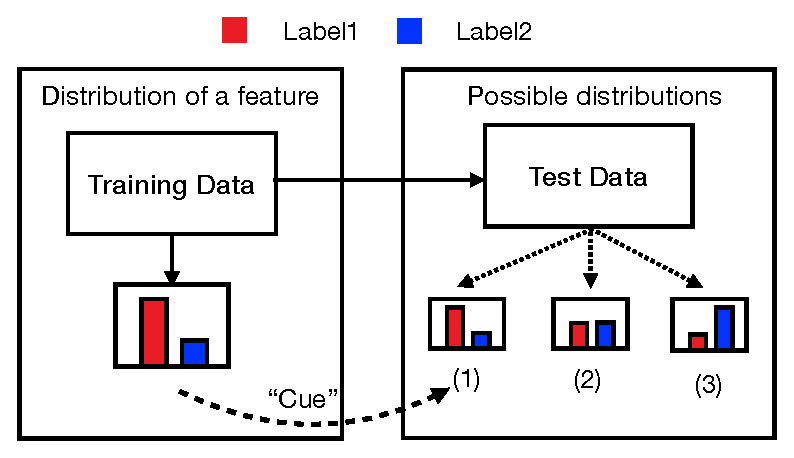
\includegraphics[width=0.6\columnwidth]{picture/cue_def.eps}
\caption{Example of a cue.}
\label{fig:cue_def}
\end{figure}

Many NL reasoning tasks can be formulated as a multiple-choice question
such as this:
\begin{example}\label{exp:snli}
An example in SNLI.\\

\noindent
\textbf{Premise}: A swimmer playing in the surf watches a low flying airplane headed inland. \\

\noindent
\textbf{Hypothesis}: Someone is swimming in the sea.\\
%\textbf{alternatives}: Entailment Contradiction  Neutral 

\noindent
\textbf{Label}: a) Entail. b) Contradict.  c) Neutral.
\end{example}
The number of candidate labels may vary. Humans solve such questions by
analyzing the logical connections between the premise and the hypothesis,
but previous work~\cite{naik2018stress,schuster2019towards} 
has found that many NLP models can solve the question
fairly well by looking only at the hypothesis (or ``conclusion'' in some work).
It is widely speculated that this is because in many datasets, 
the hypotheses are manually crafted
and may contain artifacts.
Such ``hypothesis-only'' test can identify problematic questions in the dataset
if the question can be answered correctly without looking at the premise. While
such a method is theoretically sound, 
it i) usually relies on a heavy-weight model such as Bert, which is
expensive the train and test, to achieve high detection accuracy; 
and ii) does not provide explanation why the question is a culprit.  

%Existing techniques to improve the quality of the datasets 
%include data filtering, data augmentation and stress test generation. 
%First, the data filtering model~\cite{bras2020adversarial} 
%produces a reduced dataset with fewer spurious patterns through iteratively 
%training on complex neural network models. However, 
%\KZ{Rephrase: it does't get a strongly 
%depends on the specific models to make filter decision which 
%adapts the dataset toward a few models but cannot generalize to future
%models.}
%Second, collecting more data manually for data augmentation
%is too expensive, thus some work~\cite{wang2019if,mccoy2019right} automatically generate 
%more training data in which neutralizes some 
%spurious cues with designed logic rules. 
%But these methods only focus on the word overlap problem 
%which is especially serious in certain dataset, e.g., MNLI~\cite{wang2018glue}. 
%%\KZ{What exactly do you mean by word overlap? Are we not word-overlap?}
%They can't be generalized to other datasets with different kinds of
%cues. Third, the methods~\cite{naik2018stress,mccoy2019right} 
%that generate stress test aimed at breaking the spurious cues information leakage 
%between training and testing dataset. 
%%\KZ{You mentioned cues a few sentences ago, and now you are
%%defining cues? This def is not good enough i think: 
%%We give this kind of cue a definition that if 
%%a token is unbalanced with different labels in both training and test dataset, 
%%and the distributions are similar, we will call that is a cue.
%%We illustrate this in~\figref{fig:cue_def}. 
%But the stress data generation must find 
%specific cues first and design the new dataset manually, 
%like stress test for cue ``not"~\cite{schuster2019towards}
%in ARCT dataset~\cite{niven2019probing}.
%% which is expensive.
%Few studies have focused on the description of the extent 
%to which datasets contain spurious cues, and improve these datasets 
%in a way that can benefit the evaluation of all kinds of models. 

%\KZ{I think you talk too much details in the following 4 paras.
%Cut them down to half of the size! Talk only generally, enough for ppl
%to understand at a high level!
%This para you define the kind of datasets you are targeting.}
In this paper, we propose a light-weight framework
which can be used to identify simple but effective cues 
in a broad range of multiple choice NL reasoning datasets, and thus
detect problematic question instances from a dataset. 
Though not all multiple choice questions in these dataset involve 
all three components, i.e., a premise, a hypothesis and a label, 
we will describe in~\secref{sec:approach} how to normalize them into
the standard form. In this work, we use words as the basic feature in 
constructing the spurious cues, because words are the fundamental units in
modeling natural languge in almost all modern machine learning methods.
Even more complex linguistic features such as sentiments, styles and opinions 
are built upon word features. As we will show later in the experiments,
word-based cues can track the statistical bias problems in
data set just as well as the more expensive hypothesis-only method.

%Given the instances containing premise, hypothesis and label, 
%we calculate the correlation score between cues first. 
%Different with 
%previous research which used ``hypothesis only'' method to test 
%the degree of dataset bias, we further interpret the bias feature 
%existing in ``hypothesis'' by focusing on a shallow cue, the distribution of
%words. This kind of cue may help the model obtain the correct answer 
%without truly understanding the 
%context~\cite{naik2018stress,schuster2019towards}. 
%According to Wikipedia, in linguistics, a word in spoken language can be 
%defined as a minimal phoneme sequence.
%These phonemes can be spoken in isolation and have objective or practical significance. 
%In machine learning, words are often the basic unit of semantic representation and 
%the initial semantic representation, word embedding, of most models. 
%Thus we think that even if the spurious features in the dataset 
%are the imbalance distribution of abstract features, 
%such as polarity, sentiment, etc., 
%the basically reason is still the imbalanced distribution of words.
%%\KZ{the above is very important statement. Need some backup in experiments
%%or evidence.} 
%%Word distribution balance is a sufficient and unnecessary condition for a balance dataset. 
%%In other words, when the distribution is relatively balanced, 
%%\KZ{is this too strong a statement? 
%%we can confirm that there is no imbalance problem in the dataset.}
%%When the distribution is unbalanced, we need to further use ``hypothesis only'' 
%%method to confirm.  \KZ{But how do we know it's still imbalanced after 
%%the dataset passes our cue test? It sounds like one always needs to apply
%%the hypothesis only test to confirm.}
%The reason why we don't use ``hypothesis only'' 
%directly is that, first of all, our method is very light, the representation 
%vectors have extremely low dimensions. 
%Second, our method is explicit and interpretable. It can not only show whether there is a problem in the dataset, 
%but also show problematic words.
%% We can modify these words in a certain direction.
%%Detailed description about different cues is in ~\secref{sec:related}. 
%%For investigating the unbalance scores between cues and the labels,
%%we leverage several correlation methods such as point-wise mutual information(PMI).
%%\KZ{This para is about evaluating the neural models using the easy and hard
%%split of the test set.}
%%Second, by using simple linear models with the bias score of cues we can separate 
%
%Second, to  evaluate 
%the ``biasness'' and ``quality'' of the dataset, 
%we device a very simple model using only the cues to try to
%solve the questions in the dataset. 
We can further separate the test data into the easy and the hard parts 
based on whether a question can be correctly answered
using the cue features only. The relative size of hard part over the whole
data indicates the quality of the dataset (the larger the hard part, 
the better the dataset).
%\KZ{pls quickly finish the remaining part of intro. 
%The contributions part is critical.}
%Thus we can
%separate the original dataset into easy and hard part with 
%the bias score feature of cues
%any given dataset into easy and hard part
%and thus we can evaluate the ``biasness'' and ``quality'' of the dataset. 
Meanwhile, this hard-easy split can be used as a ``stress test'' to
estimate the real reasoning power of a model. 
A large difference in classification accuracy on these two parts indicates
the weakness of the model.
%using simple and cost-effective linear classification models 
%on the simple cue features,
%which trained with unbalanced score of cues to several benchmark datasets across 
%various tasks and domains. 
%We evaluate the effectiveness of our methods with the 
%deviation between our results and random selection results. 
%Simultaneously, the test set can be divided into two parts: \textbf{easy} and \textbf{hard}. 
 %\textbf{balance} and \textbf{imbalance} are relative rather than absolute. 
%\KZ{Improving the neural models by splitting the training set.} 

Finally, we propose a simple method of splitting the training data 
in to easy and hard parts, too,
and show that by filtering out the easy questions from training data,
there is a potential to improve the reasoning power of the model by ``forcing'' it
to steer its focus away from trivial cues. 

%The training data can be separated into $n$ parts, test on one part and training 
%the model on the rest for each time. 
%The filtered part contains the instances 
%which can not be correctly chosen.
%The filtered data will be used to train a better model for target tasks. 

In summary, this paper makes the following contributions:
%\KZ{These contribs need to be revised right?}
\begin{itemize}
\item We provide a light-weight but effective method to evaluate to what extent 
multiple choice datasets are infected with information leaks of spurious statistical
cues and to pinpoint what exactly these cues are 
(\secref{sec:approach}, \secref{sec:experiment1}).
%(\secref{sec:result}).

\item By splitting the test data into two parts according to  
the severity of information leaks, 
we can estimate a given model's true ability to reason
by the difference in its performance on the easy and hard 
part~(\secref{sec:experiment2}).

\item We further split the training set using a heuristics that allows to
train the model to better accuracy on the hard test data (\secref{sec:experiment3}). 
\end{itemize}
% (\secref{sec:result}).

%\item We filter the training data and get a better performance on the \textbf{hard} dataset.
%to get a high quality training dataset which
 %is possibly closer to the intended task. 

















